\documentclass[11pt]{article}
\usepackage[margin=1in]{geometry}
\usepackage{fancyhdr}
\usepackage[T1]{fontenc}
\usepackage[utf8]{inputenc}
\usepackage{lmodern}
\usepackage{microtype}
\usepackage{csquotes}
\usepackage{booktabs}
\usepackage{enumitem}
\usepackage{fvextra}
\usepackage{tikz}
\usetikzlibrary{positioning}
\usepackage[colorlinks=true,linkcolor=black,citecolor=black,urlcolor=blue]{hyperref}
\hypersetup{pdftitle={The Casino Is Not the Building: Transaction Topology and the Boundaries of Virtual Worlds},pdfauthor={Watson Hartsoe},pdfsubject={Virtual worlds, loot boxes, platform governance, and transaction topology},pdfkeywords={virtual worlds, loot boxes, gambling, platform governance, metaverse, interoperability}}
\usepackage[backend=biber,style=authoryear,maxcitenames=2]{biblatex}
\addbibresource{the-casino-in-the-fountain__references.bib}
\setlength{\parindent}{0pt}
\setlength{\parskip}{0.65em}
\title{The Casino Is Not the Building:\\Transaction Topology and the Boundaries of Virtual Worlds}
\author{Watson Hartsoe}
\date{17 August 2026}
\pagestyle{fancy}
\fancyhf{}
\fancyhead[L]{\footnotesize The Casino Is Not the Building}
\fancyhead[R]{\footnotesize Watson Hartsoe}
\fancyfoot[C]{\thepage}
\newcommand{\aimark}{\tikz[baseline=-0.7ex,scale=.18]{\draw[line width=.55pt,line cap=round] (0,0) circle (.10);\draw[line width=.45pt,line cap=round] (-.055,-.015) .. controls (0,-.07) and (.055,-.07) .. (.075,-.015);\draw[line width=.7pt,line cap=round] (.18,-.14) arc[start angle=-38,end angle=55,radius=.28];\draw[line width=.7pt,line cap=round] (.31,-.25) arc[start angle=-39,end angle=56,radius=.46];\draw[line width=.7pt,line cap=round] (.46,-.37) arc[start angle=-40,end angle=57,radius=.66];}}
\setlength{\headheight}{14pt}

\begin{document}
\begin{titlepage}
\centering
\vspace{1.05in}
{\LARGE\bfseries The Casino Is Not the Building\par}
\vspace{0.2in}
{\Large Transaction Topology and the Boundaries of Virtual Worlds\par}
\vfill
{\large Watson Hartsoe\par}
\vspace{0.12in}
{\normalsize 17 August 2026\par}
\vfill
{\footnotesize Working Paper\par}
\begin{tikzpicture}[remember picture,overlay]
  \node[anchor=south east,align=right,text width=3.1in] at ([xshift=-0.55in,yshift=0.45in]current page.south east)
  {\scriptsize \aimark\quad \\textbf{Working Paper · AI-augmented research process}\\[-1pt]
   \tiny Evidence, prompts, and making history preserved.};
\end{tikzpicture}
\end{titlepage}

\begin{abstract}
Research on loot boxes and gambling-like mechanics often begins with conspicuous objects: crates, wheels, slot machines, or casino-themed rooms. This paper argues that the more stable unit of analysis is not the visual object or the three-dimensional place but a distributed \emph{transaction topology}: the chain connecting consideration, randomization, mapping, reward, inventory state, transferability, cash-out, jurisdiction, and platform policy. A comparative reading of virtual-world and platform documentation shows why this shift matters. Kaneva and Mozilla Hubs demonstrate that one world can be exposed through multiple representational surfaces; Roblox shows policy becoming player-specific runtime state and a random purchase becoming diegetic ``fountain'' physics; Minecraft makes non-interoperability an economic safety condition; Second Life makes convertibility and jurisdiction spatially consequential; and Xsolla exposes commerce and loot-box operations as metadata and API transitions outside the rendered scene. The resulting claim is that the boundary of a virtual world can participate in the gambling mechanism itself. Regulation and audit should therefore trace value and permissions across system boundaries rather than classify mechanics by their visual skin alone.
\end{abstract}

\textbf{Keywords:} virtual worlds; loot boxes; gambling; platform governance; metaverse; interoperability; game economies; transaction topology

\section{Introduction: the wrong object}
A casino is easy to recognize when it looks like a casino. A slot machine, roulette wheel, or treasure chest appears to supply the analyst with a ready-made unit of inquiry. Yet platform rules themselves repeatedly undermine this visual shortcut. Linden Lab's wagering policy explicitly states that its concern does not depend on whether an activity sits in a building called an in-world casino \parencite{linden_wagering_policy}. Roblox, meanwhile, explains its random-virtual-item rules with an example in which a player acquires a virtual marble and throws it into a fountain to receive a random item \parencite{roblox_marble_fountain_2026}. The first case strips architecture from the classification; the second shows a transaction reappearing as environmental action.

This paper develops a simple proposition: \emph{the casino is not the building}. Gambling-like mechanics in virtual environments are better described as relations among operations than as places or props. Consideration may occur on a web checkout page, randomization may be handled by a service, the reward may materialize in a three-dimensional scene, cash-out may exist only for a creator rather than a player, and jurisdictional restrictions may be evaluated through an API. What the player experiences as one event may therefore be assembled across several interfaces and institutions.

I call this assembly a \emph{transaction topology}. The term does not propose a new legal test for gambling. Rather, it names an analytical representation capable of keeping together operations that visual analysis tends to separate: payment, chance, mapping, entitlement, convertibility, policy, and state change. This representation is particularly important for virtual worlds because their operational boundaries rarely coincide with the edges of the rendered scene.

\section{From rendered worlds to persistent systems}
The first step is to loosen the identification of ``virtual world'' with ``3D scene.'' Kaneva described movement between its two-dimensional web and its three-dimensional virtual world as part of one service experience \parencite{norris2009virtualhealth}. Mozilla Hubs intensified this pattern by making a room directly addressable through a URL and accessible across desktop, mobile, and immersive hardware \parencite{white2018hubs}. Hubs also allowed pasted web resources to become manipulable objects in a shared room \parencite{marinacci2018hubsmedia}. In such systems, dimensionality is a property of a rendering or interface, not necessarily of the persistent social referent.

This observation matters for platform economies. A purchase can leave the rendered game while remaining inside the game's operational world. Xsolla's web-shop infrastructure, for example, describes browser-based checkout for virtual items and currencies that are synchronized back into game state \parencite{xsolla2025buybutton}. The player may visually ``leave'' the game to pay, but the transaction remains part of the same entitlement system. Conversely, a URL can become a room or an object. The two-dimensional web and the three-dimensional scene are not separate ontological domains so much as different surfaces through which world state is addressed and transformed.

A useful abstraction is therefore:
\begin{center}
\texttt{WORLD STATE -> REPRESENTATION / SERVICE -> OPERATION -> WORLD STATE'}.
\end{center}
The world includes identity, inventory, permissions, currency, social relations, and histories even when those are administered outside the 3D scene. This is the paper's deliberately strange stepping stone: Mozilla Hubs' conversion of a URL into a movable room object is not about gambling at all, yet it makes visible the broader operation by which information acquires spatial affordances. Once that transformation is legible, a loot box can be understood in the opposite direction: a spatial metaphor can be stripped back into the informational state transition that it performs.

\section{The transaction below the skin}
Gambling regulation already contains a language for decomposing apparently unified games. The UK Gambling Commission's remote technical standards distinguish generation of random outcomes from the mapping of generated values into game outcomes \parencite{ukgc_rts7_random_outcomes,ukgc_rts7_mapping}. Its guidance on remote gambling equipment similarly treats gambling systems as assemblies of equipment that perform different operations \parencite{ukgc_remote_gambling_equipment}. A fair-looking animation is therefore not the mechanism in full, and a valid random-number generator does not by itself establish a fair mapping from numbers to consequences.

The same decomposition becomes almost literal in infrastructure APIs. Xsolla historically exposed an endpoint whose operation was to open a loot box in a user's game inventory \parencite{xsolla_open_lootbox_api}. At that layer the chest has disappeared. There is no lid, particle effect, avatar hand, or casino room--only an authenticated request and a state mutation. The representational skin is optional from the perspective of the backend operation.

This suggests a transaction-topology model with at least six separable positions:
\begin{enumerate}[nosep]
\item \textbf{consideration}: what the user commits;
\item \textbf{randomization}: how contingency is produced;
\item \textbf{mapping}: how random values become possible outcomes;
\item \textbf{entitlement}: how the result becomes inventory or access;
\item \textbf{transfer}: where the resulting value may move;
\item \textbf{policy}: which actor, jurisdiction, or platform conditions permit the preceding operations.
\end{enumerate}
A treasure chest, fountain, wheel, or plain button can all be interfaces onto the same topology. Conversely, two visually identical chests can belong to different topologies if one reward is transferable or cashable and the other is not.

\begin{figure}[ht]
\centering
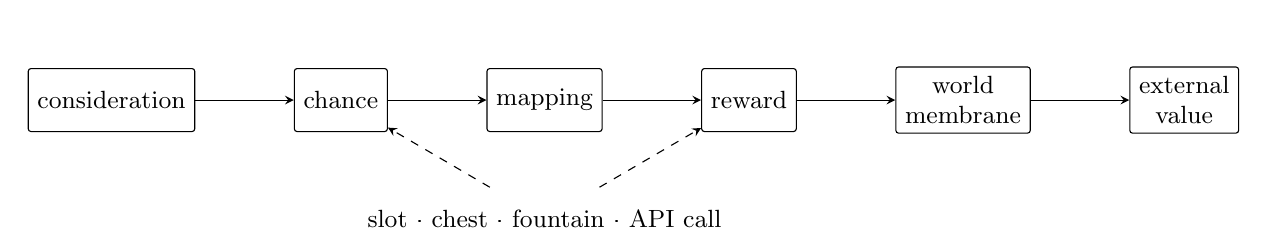
\begin{tikzpicture}[>=stealth,every node/.style={draw,rounded corners=1pt,align=center,font=\small,minimum height=.8cm}]
\node (pay) {consideration};
\node (chance) [right=1.25cm of pay] {chance};
\node (map) [right=1.25cm of chance] {mapping};
\node (reward) [right=1.25cm of map] {reward};
\node (membrane) [right=1.25cm of reward] {world\\membrane};
\node (value) [right=1.25cm of membrane] {external\\value};
\draw[->] (pay)--(chance);\draw[->] (chance)--(map);\draw[->] (map)--(reward);\draw[->] (reward)--(membrane);\draw[->] (membrane)--(value);
\node[draw=none,below=.7cm of map] (skin) {slot · chest · fountain · API call};
\draw[dashed,->] (skin)--(chance);\draw[dashed,->] (skin)--(reward);
\end{tikzpicture}
\caption{Transaction topology separates the operational chain from its diegetic skin.}
\end{figure}

\section{The world membrane is part of the mechanism}
The strongest consequence of this model is that the ``boundary of the game'' is not merely a container around the mechanic. It can alter the mechanic's regulatory and economic meaning. In its 2022 response on loot boxes, the UK government observed that most loot boxes did not meet the Gambling Act definition because prizes were confined to the game and could not be converted into real-world money, while also noting evidence of association between loot-box purchasing and problem gambling \parencite{dcms2022lootboxes}. The key point here is not that non-cashable loot boxes are harmless; the government explicitly did not establish that. It is that convertibility is load-bearing in the legal analysis.

Platform policies reproduce this concern as technical boundaries. Linden Lab distinguishes chance-based payouts involving non-convertible novelty objects from payouts that can readily become Linden dollars, real currency, or other value \parencite{linden_wagering_policy}. Minecraft permits server currencies under conditions that include no cash-out, no real-world conversion, and no transfer across servers \parencite{minecraft_usage_guidelines_2026}. What looks like a defect from the perspective of ``open metaverse'' interoperability--a currency that fails to travel--is here a governance feature.

Roblox complicates any binary notion of convertibility. Players can purchase Robux and spend them on virtual products, while qualifying creators may convert certain \emph{Earned Robux} into real currency through the Developer Exchange program \parencite{roblox_devex_2026}. Convertibility is thus actor- and provenance-dependent. Asking whether ``Robux can cash out'' is too coarse. A better question is which units, earned by whom, through which path, are eligible to cross the membrane.

The membrane should therefore be modeled as a graph of permitted transformations rather than a single inside/outside line. Two systems can expose the same purchase and random-reward animation while differing only in one downstream edge--for example, player-to-player resale or fiat conversion. That edge may be invisible at the moment of play yet decisive for economic classification.

\section{Law becomes world state}
Virtual-world governance also demonstrates that policy can be compiled into the world rather than merely written around it. Roblox's PolicyService returns player-specific policy information based on factors including location, age group, and platform, enabling an experience to alter mechanics at runtime \parencite{roblox_policyservice}. The practical result is striking: two avatars co-present in the same rendered room can inhabit different executable possibility spaces.

Second Life produces a spatial variant of the same phenomenon. Linden Lab's Skill Gaming Policy conditions access to designated regions on legal age, account requirements, and authorized jurisdiction \parencite{linden_skill_policy}. Jurisdiction is converted into reachability. The virtual map is therefore not identical for every resident; lawful entry is relational between person and place.

Xsolla moves policy to yet another layer. Its catalog-management documentation includes a ``paid randomized reward'' marking for currencies, items, packages, or bundles participating in loot-box or gacha mechanics and notes jurisdictional legal restrictions around such mechanics \parencite{xsolla_catalog_randomized_reward}. Here the regulatory category becomes product metadata. Across these cases law appears as a player property, a spatial gate, and an object annotation. The common transformation is from prose rule to executable condition.

This suggests a broader design concept: \emph{legal geometry}. A rendered world may appear shared while its available actions, regions, products, or transactions are selectively generated for different users. The operative geography of the world is therefore a function of policy, not only coordinates.

\section{Diegetic camouflage and operational equivalence}
The distinction between transaction and representation becomes especially important when randomized purchases are made diegetic. Roblox's marble-and-fountain example translates an economic-probabilistic operation into objects and causal gestures \parencite{roblox_marble_fountain_2026}. The user does not merely press ``buy random item''; the system can represent the action as acquiring a marble, throwing it, and receiving an outcome from the environment.

Nothing in the cited Roblox documentation establishes that this representation causes greater spending or confusion. That behavioral claim would require evidence the present corpus does not contain. The analytical point is narrower: the same transaction class can be represented through an ordinary-looking world action. Visual inspection alone therefore cannot establish operational equivalence or difference.

A practical audit could test this directly by implementing one invariant backend transaction behind multiple interfaces: slot machine, treasure chest, pet egg, fountain, tree harvest, and plain button. The price, outcome distribution, reward inventory, and transfer rules would remain constant. Researchers could then separately measure (1) whether users recognize price and probability, and (2) whether policy systems classify the implementations identically. Such a design would distinguish the effect of \emph{skin} from the effect of \emph{topology}.

\section{Observability is itself a governance problem}
The 2022 UK government review identified a stable association between loot-box purchasing and problem gambling but concluded that the available evidence did not establish a causal relationship; it also identified access to industry and player data as a barrier to research \parencite{dcms2022lootboxevidence}. Transaction topology sharpens why this matters. Platforms can often observe the sequence of events needed to discriminate mechanisms: purchase amount, odds table, acquisition time, session context, user segment, inventory changes, and subsequent transactions. External researchers may see only surveys or partial behavioral traces.

The platform may therefore possess not only the mechanic but also the best instrument for observing it. This asymmetry matters for governance because regulation directed at visual categories cannot substitute for access to operational traces. If a chest, fountain, and API request can implement related state transitions, then audit must follow event and value flows across interfaces.

\section{Implications}
Three implications follow.

First, \textbf{regulation should target operations before skins}. Platform rules already do this in part: Linden Lab's wagering policy ignores casino architecture, Roblox conditions random-item transactions, and Xsolla marks randomized-reward participation in catalog metadata. A transaction-graph representation could make those similarities explicit.

Second, \textbf{interoperability is not unconditionally desirable}. The Minecraft case demonstrates that preventing currency from crossing server or cash boundaries can be a deliberate safety condition. Open-world design should therefore ask not only which objects \emph{can} travel but which transformation edges ought to remain impossible.

Third, \textbf{the relevant world extends beyond the executable scene}. Checkout pages, policy APIs, billing descriptors, support routes, creator cash-out systems, and source repositories are not peripheral to virtual-world governance. They are organs of the operational world. This is why the Hubs and Kaneva lineage matters to gambling analysis: once the world is understood as persistent referential and transactional state rather than simply a 3D place, the apparently external web page or API can be seen as part of the same system of consequence.

\section{Limitations}
This paper is a conceptual synthesis of a bounded source collection rather than a jurisdiction-wide legal analysis. Platform terms and policies differ across jurisdictions and change over time. The comparison among UK government materials, Linden Lab, Roblox, Minecraft, and Xsolla therefore does not establish one universal definition of gambling.

The paper also does not establish that diegetic representations such as fountains or treasure chests causally change user behavior. It identifies an audit problem and proposes a comparative test. Likewise, cross-interface continuity in Kaneva and Hubs should not be generalized to mean that every object or capability is invariant across every client.

Finally, the source corpus is asymmetric. Platform documentation reveals some APIs and policy predicates but not all implementation details. Xsolla's deprecated loot-box endpoint, for example, exposes an opening operation but does not establish where random selection occurred internally \parencite{xsolla_open_lootbox_api}. Transaction topology should therefore be treated as a method for locating missing variables as much as for describing known ones.

\section{Conclusion}
The central claim can be stated compactly: the casino is not the building because the mechanism is distributed. Chance can live in an RNG service, meaning in an outcome map, payment in a web checkout, entitlement in an inventory service, law in a policy boolean, jurisdiction in a spatial gate, and value in the existence of an exit path from the world. A three-dimensional interface may stage those operations as one coherent event, but the coherence is representational rather than architectural.

For research on virtual-world economies, the useful unit is therefore not the chest, wheel, room, or platform screen taken in isolation. It is the path along which state and value transform. The virtual-world boundary belongs inside that model because it can determine which transformations remain possible. The same world that gives a hyperlink a body can give a transaction a fountain; the analytical task is to follow the operation through both transformations.

\printbibliography



\clearpage
\appendix
\sloppy
\section{Assembly Instrument}
The publication assembly instrument is preserved verbatim outside the manuscript so that the scholarly argument does not become a reproduction of its own compiler instructions. The exact text is available at \path{_PROMPTS/10__slipcase-v15.55-AM__assembly.poml} and in the sibling file \path{the-casino-is-not-the-building__ASSEMBLY_APPENDIX.txt}. Its SHA-256 is \texttt{a5ef0e2e3ea56463e25065f19e7313b4}\linebreak\texttt{e9c8c569b8cceb1a3c5d9f05bd83598a}. The same instrument is embedded in \path{index.html}.

\section{Making History}
This paper is derived interpretation, not canonical evidence. The 33 archived zettel payloads were inherited unchanged from a prior verified checkpoint. The research steward supplied the source materials, research prompts, and the current SLIPCASE assembly instrument. The model compiled relations, selected and developed the paper's argument, wrote connective prose, and produced derived interfaces. Deterministic tools computed hashes, counts, graph statistics, citation checks, PDF build status, and ZIP integrity. A fuller account is preserved in \path{000__MAKING_HISTORY.txt} and \path{the-casino-is-not-the-building__MAKING_HISTORY.txt}. No human peer review is claimed.

\section{Replication Path}
A recipient without access to the originating conversation can begin with \path{index.html}, then inspect \path{000__RETURN_PATH.txt}, \path{000__REBUILD.txt}, the exact zettel deck, machine-readable graph files under \path{_SLIPCASE/}, preserved prompts under \path{_PROMPTS/}, and resources under \path{_RESOURCES/}. Paper claims are traced back to zettels and sources in \path{the-casino-is-not-the-building__SOURCE_MAP.txt}. The compiled bibliography is \path{the-casino-in-the-fountain__references.bib}.

\end{document}
